\documentclass[11pt]{article}
\usepackage{xspace,epsfig,amsmath,amsthm,amssymb,fullpage}
\topmargin   0pt
\marginparwidth 0pt
\oddsidemargin  0pt
\evensidemargin 0pt
\marginparsep 0pt
\textwidth   6.5in
\textheight  9.2in

\usepackage{tikz}
\usepackage{tikz-qtree,tikz-qtree-compat} % for parse trees

\usepackage{latexsym}
\usepackage{amssymb}
\usepackage{amsmath}
\usepackage{amsthm}
\usepackage{amsfonts}
\usepackage{bm} 
% \usepackage{prooftree}
\usepackage{flagderiv}
\usepackage{logicproof}
\usepackage{bussproofs}
\usepackage{hyperref}
\usepackage{color}
\usepackage{listings}
\usepackage{synttree} 
\usepackage{pdflscape}
\usepackage{enumitem}
\usepackage{multicol}

\definecolor{keywordcolor}{rgb}{0.7, 0.1, 0.1}   % red
\definecolor{tacticcolor}{rgb}{0.0, 0.1, 0.6}    % blue
\definecolor{commentcolor}{rgb}{0.4, 0.4, 0.4}   % grey
\definecolor{symbolcolor}{rgb}{0.0, 0.1, 0.6}    % blue
\definecolor{sortcolor}{rgb}{0.1, 0.5, 0.1}      % green
\definecolor{attributecolor}{rgb}{0.7, 0.1, 0.1} % red

\def\lstlanguagefiles{lstlean.tex}
% set default language

\hypersetup{colorlinks=true,linkcolor=blue,urlcolor=blue}
% WARNING:
% Do NOT use package `bussproofs' and package `prooftree' at the same time,
% \begin{prooftree} ... \end{prooftree} is an environment defined in the
% package  `bussproofs', which conflicts with the name of the package
% `prooftree'.

\newcommand{\defn}{\overset{\text{\scriptsize def}}{=}}
\newcommand{\Intro}[1]{{#1}{\text{i}}}
\newcommand{\IntroA}[1]{{#1}{\text{i}_1}}
\newcommand{\IntroB}[1]{{#1}{\text{i}_2}}
\newcommand{\Elim}[1]{{#1}{\text{e}}}
\newcommand{\ElimA}[1]{{#1}{\text{e}_1}}
\newcommand{\ElimB}[1]{{#1}{\text{e}_2}}
\newcommand{\Set}[1]{\{ #1 \}}
\newcommand{\SET}[1]{\Bigl\{ #1 \Bigr\}}
\newcommand{\TTT}{\bm{\mathsf{T}}}
\newcommand{\FFF}{\bm{\mathsf{F}}}
\setlength{\parindent}{0pt}
% parameters: four corners, title, scribes' names
\newcommand{\handout}[6]{{
\begin{center}
\begin{minipage}{14cm}
    \setlength{\parindent}{0cm}%
    \fbox{\vbox{%
        {#1}%
        \hfill
        #2

        \center{\Large\bf{#5}}

        \emph{#3}\hfill #4
    }}%
    \vskip0pt
    \vbox{\hfill  #6}%
\end{minipage}
\\ 
\end{center}
}}

%%%%%%%%%%%%%%%%%%%%%%%%%%%%%%%%%%%%%%%%%%%%%%%%%%%%%%%%%%%%%%%%%%%%%%

\begin{document}
\handout{CS 511 Formal Methods, Fall 2024}
        {Instructor: Assaf Kfoury}
        {December 12, 2024}
        {Lucas Miguel Tassis}
        {Homework Assignment 13}

%%  THE FOLLOWING IS USED WITH THE logicproof ENVIRONMENT:
%%
\setlength{\subproofhorizspace}{.5em}
\setlength{\intersubproofvertspace}{0.5em}
\lstset{language=lean}


\section*{Exercise 1} 

\begin{enumerate}[label=(\alph*)]
    \item First-order logic is sufficient for most of the basic SQL operations. Most of the SQL operations such as \texttt{SELECT}, \texttt{GROUPBY}, \texttt{JOIN}, in addition to the \texttt{EXISTS} operation mentioned in the exercise are first-order definable. More generally, relational algebra, which is the theoretical foundation of most relational databases is first-order definable\footnote{Reference: \href{https://simons.berkeley.edu/sites/default/files/docs/5225/simons162.pdf}{Logic and Databases by Phokion G. Kolaitis}}. However, some more complex operations present in newer database systems might need the use of second-order logic (such as operations over sets and their subsets, \emph{e.g.} queries about all subsets).
    \item The diagram that represents the schema is:
        \begin{figure*}[h] 
            \centering
            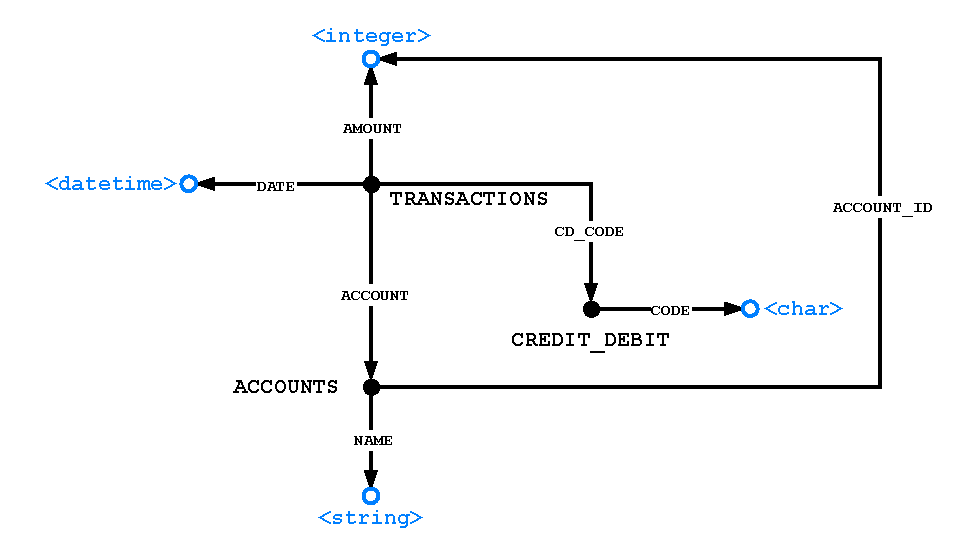
\includegraphics{hw13-category.pdf}
        \end{figure*}
\end{enumerate}


\section*{Exercise 2}

\begin{enumerate}[label=(\alph*)]
    \item The 19 morphisms of $\mathcal{K}$ are:
    \begin{multicols}{3}
        \begin{enumerate}[label=(\arabic*)]
            \item $f : A \to B$
            \item $h : A \to C$
            \item $i : A \to D$
            \item $g : B \to A$
            \item $k : B \to C$
            \item $j : D \to A$
            \item $\ell : D \to C$
            \item $\mathrm{id}_{A} : A \to A$
            \item $\mathrm{id}_{B} : B \to B$
            \item $\mathrm{id}_{C} : C \to C$
            \item $\mathrm{id}_{D} : D \to D$
            \item $f\circ  k : A \to C$
            \item $i\circ  \ell : A \to C$
            \item $g\circ  h : B \to C$
            \item $g\circ  i : B \to D$
            \item $j\circ  f : D \to B$
            \item $j\circ  h : D \to C$
            \item $(g \circ i) \circ \ell : B \to C$
            \item $(j \circ f) \circ k : D \to C$ 
        \end{enumerate}
    \end{multicols}
    \item The list of morphisms of $\mathcal{K}'$ is:
    \begin{multicols}{3}
        \begin{enumerate}[label=(\arabic*)]
            \item $\mathrm{id}_{A}' : A \to A$
            \item $\mathrm{id}_{B}' : B \to B$
            \item $\mathrm{id}_{C}' : C \to C$
            \item $\mathrm{id}_{D}' : D \to D$
            \item $f' : A \to B$
            \item $h' : A \to C$
            \item $i' : A \to D$
            \item $g' : B \to A$
            \item $k' : B \to C$
            \item $j' : D \to A$
            \item $\ell' : D \to C$
            \item $(g\circ i)' : B \to D$
            \item $(j\circ f)' : D \to B$            
        \end{enumerate}
    \end{multicols}
    Notice that these morphisms cover all the domains and codomains present in $\mathcal{K}$, just eliminating the redundancy. 
    \item First, recall that the properties of a functor are:
    \begin{enumerate}[label=(\arabic*)]
        \item Objects to objects;
        \item Morphisms to morphisms;
        \item Respect the identity;
        \item Respect composition.
    \end{enumerate}
    Therefore, we can define a functor $F : \mathcal{V} \to \mathcal{K}$:
    \begin{enumerate}[label=(\arabic*)]
        \item $F(U) = B$, $F(W) = D$, and $F(V) = C$;
        \item $F(p) = k$ and $F(q) = \ell$;
        \item $F(\mathrm{id}_{U}) = \mathrm{id}_{B}$, $F(\mathrm{id}_{W}) = \mathrm{id}_{D}$, and $F(\mathrm{id}_{V}) = \mathrm{id}_{C}$
    \end{enumerate}
    \begin{figure}[h]
        \centering
        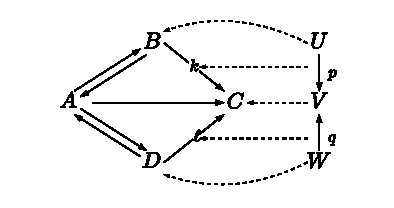
\includegraphics[scale=1.5]{hw13-functor.pdf}
    \end{figure}

    \item Because in this category we have four vertices and all vertices have outgoing connections. If we look at $\mathcal{K}$, the vertex $C$ is a sink (\emph{i.e.} it has no outgoing connections). Therefore, there cannot exist a functor from this category to $\mathcal{K}$, because there is not a mapping for $C$, violating the functor properties.
\end{enumerate}


\section*{Exercise 3}
The Lean template file with the solutions is available on \href{https://github.com/lucastassis/BU-CS511/blob/main/HW13/code/HW13.lean}{GitHub}.

\section*{Exercise 4}
The Lean template file with the solutions is available on \href{https://github.com/lucastassis/BU-CS511/blob/main/HW13/code/HW13.lean}{GitHub}.

\section*{Problem 2}
The Lean template file with the solutions is available on \href{https://github.com/lucastassis/BU-CS511/blob/main/HW13/code/HW13.lean}{GitHub}.




\end{document}
